%%%%%%%%%%%%%%%%%%%%%%%%%%%%%%%%%%%%%%%%%
% fphw Assignment
% LaTeX Template
% Version 1.0 (27/04/2019)
%
% This template originates from:
% https://www.LaTeXTemplates.com
%
% Authors:
% Class by Felipe Portales-Oliva (f.portales.oliva@gmail.com) with template 
% content and modifications by Vel (vel@LaTeXTemplates.com)
%
% Template (this file) License:
% CC BY-NC-SA 3.0 (http://creativecommons.org/licenses/by-nc-sa/3.0/)
%
%%%%%%%%%%%%%%%%%%%%%%%%%%%%%%%%%%%%%%%%%

%----------------------------------------------------------------------------------------
%	PACKAGES AND OTHER DOCUMENT CONFIGURATIONS
%----------------------------------------------------------------------------------------

\documentclass[
  french,
  % twocolumn,
	11pt, % Default font size, values between 10pt-12pt are allowed
	%letterpaper, % Uncomment for US letter paper size
	%spanish, % Uncomment for Spanish
]{fphw}

% \usepackage[fontsize=10.0]{scrextend} % Use this to force the fontsize

%% Commands for numbering paragraphs
\renewcommand\thesection{\Roman{section}}
\renewcommand\thesubsection{\thesection.\arabic{subsection}}
\renewcommand*\thesubsubsection{%
  \Roman{section}.\arabic{subsection}.\alph{subsubsection}%
}

\usepackage{sectsty}
\sectionfont{\bfseries\Large\raggedright}

% Template-specific packages
\usepackage{babel}
\usepackage[utf8]{inputenc} % Required for inputting international characters
% \usepackage{DejaVuSerifCondensed} 
\usepackage[T1]{fontenc} % Output font encoding for international characters

\usepackage{kpfonts}        %% For math only
\usepackage{fontspec}       %% Because we are using XeTEX
\setromanfont{Minion Pro}   %% For text (Minion Math is commercial)

%-----------------------------------------------------------------------
% \setromanfont{Meta Serif Pro}
% \setsansfont{Fira Sans}
% \setmonofont[Color={0019D4}]{Fira Code} 
%-----------------------------------------------------------------------

\usepackage{fancyvrb}
\usepackage{fvextra}
\newcommand\userinput[1]{\textbf{#1}}
\newcommand\arguments[1]{\textit{#1}}

\usepackage{amsmath}
\usepackage{mathtools}
\usepackage{xfrac} 

\usepackage{graphicx} % Required for including images
\usepackage[textfont=it,font=small]{caption}  %% To manage long captions in images
\usepackage{subcaption}
\captionsetup{justification=centering}

\usepackage{float}
\graphicspath{ {../img/} }

\usepackage{booktabs} % Required for better horizontal rules in tables

\usepackage{listings} % Required for insertion of code

\usepackage{array} % Required for spacing in tabular environment

\usepackage{enumerate} % To modify the enumerate environment

\usepackage{amssymb}
\usepackage{enumitem}	%% % To modify the itemize bullet character

\newcommand{\tabhead}[1]{{\bfseries#1}}

\usepackage{xcolor}
\usepackage{listings}
\colorlet{mygray}{black!30}
\colorlet{mygreen}{green!60!blue}
\colorlet{mymauve}{red!60!blue}
\lstset{
  backgroundcolor=\color{gray!10},  
  basicstyle=\ttfamily,
  columns=fullflexible,
  breakatwhitespace=false,      
  breaklines=true,                
  captionpos=b,                    
  commentstyle=\color{mygreen}, 
  extendedchars=true,              
  frame=single,                   
  keepspaces=true,             
  keywordstyle=\color{blue},      
  language=c++,                 
  numbers=none,                
  numbersep=5pt,                   
  numberstyle=\tiny\color{blue}, 
  rulecolor=\color{mygray},        
  showspaces=false,               
  showtabs=false,                 
  stepnumber=5,                  
  stringstyle=\color{mymauve},    
  tabsize=3,                      
  title=\lstname                
}

\usepackage[linkcolor=blue,colorlinks=true]{hyperref}
% \usepackage[colorlinks=true,urlcolor=blue]{hyperref}
\hypersetup{citecolor=blue}

\usepackage{cleveref}
\usepackage{siunitx}
\usepackage{bm}

\usepackage[backend=bibtex,style=alphabetic,maxnames=2,natbib=true]{biblatex} % Use the bibtex backend with the alphabetic citation style (compact APA-like)
% \usepackage[backend=bibtex,style=authoryear,maxnames=2,natbib=true]{biblatex} % Use the bibtex backend with the authoryear citation style (which resembles APA)
\addbibresource{../bib/bibliography.bib} % The filename of the bibliography
\usepackage[autostyle=true]{csquotes} % Required to generate language-dependent quotes in the bibliography 
% \renewcommand*{\bibfont}{\tiny} % Pour reduire la taille des references

\usepackage[useregional=numeric]{datetime2}
\usepackage[normalem]{ulem}

% %-------------------------------------------------------------------------------

\newcommand{\myvec}[3]{\begin{pmatrix} #1  \\ #2 \\ #3 \end{pmatrix}}   %% vecteur 3d
\newcommand{\mymat}[9]{\begin{pmatrix} #1 & #2 & #3 \\ #4 & #5 & #6 \\ #7 & #8 &#9 \end{pmatrix}}  %% Matrice 3*3

\renewcommand{\vector}[4]{\begin{pmatrix} #1  \\ #2 \\ #3 \\ #4 \end{pmatrix}}   %% vecteur 4d
% \newcommand{\mymatrix}[16]{\begin{pmatrix} #1 & #2 & #3 & #4 \\ #4 & #6 & #7 & #8 \\ #9 & #10 & #11 & #12 \\ #13 & #14 & #15 & #16 \end{pmatrix}}  %% Matrice 3*3

\newcommand{\hquad}{\hspace{0.5em}} %% Bew command for half quad
\newcommand*\diff{\mathop{}\!\mathrm{d}}
% \setlength\parindent{0pt}	%% To remove all indentations
\newcommand{\bvec}[1]{\bm{\mathrm{#1}}}  %% Use this to make vectors
\newcommand{\bmat}[1]{\bm{\mathsf{#1}}}   %% Use this to make tensors

%----------------------------------------------------------------------------------------
%	ASSIGNMENT INFORMATION
%----------------------------------------------------------------------------------------

\title{Compte rendu semaine \#11} % Assignment title
% \title{Difficultés rencontrées} % Assignment title

\author{Roussel Desmond Nzoyem} % Student name

\date{\DTMdisplaydate{2021}{4}{13}{-1} - \DTMdisplaydate{2021}{4}{20}{-1}} % Due date

\institute{Sorbonne Université \\ Laboratoire Jacques-Louis Lions} % Institute or school name

\class{Stage M2} % Course or class name

\professor{Pr. Stéphane Labbé} % Professor or teacher in charge of the assignment

%----------------------------------------------------------------------------------------

\begin{document}

\maketitle % Output the assignment title, created automatically using the information in the custom commands above

%----------------------------------------------------------------------------------------
%	ASSIGNMENT CONTENT - INTRO
%----------------------------------------------------------------------------------------

Le travail de cette semaine fut lié à l'animation du modèle 1D pour observer comment un floe rebondit après contact avec un autre floe. Je me suis aussi penché sur la question des conditions nécessaires d'existence de solution pour la modélisation d'un floe isolé (voir \cref{fig:dep1d}).

\begin{figure}[H]
  \centering
  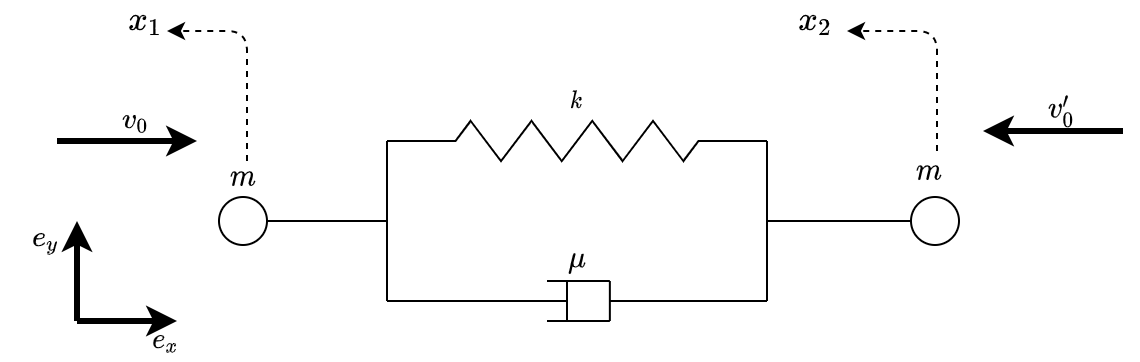
\includegraphics[width=.6\textwidth]{Deplacement1D-Systeme.png}
  \caption{Déplacement 1D (nécessaire pour la deuxième phase de l'animation).}
  \label{fig:dep1d}
\end{figure}




%----------------------------------------------------------------------------------------
%	ASSIGNMENT CONTENT - SECTION 1
%----------------------------------------------------------------------------------------

\section*{Tâches effectuées}

La principale tâche effectuée à été l'animation du modèle de percussion 1D. J'ai divisé cette partie en deux phase:
\begin{enumerate}
    \item \textbf{Avant le contact}: pour faciliter les travaux, je suppose que les floes sont en mouvement rectilignes uniformes (voir \cref{fig:anim1}).
    \begin{figure}[H]
      \centering
      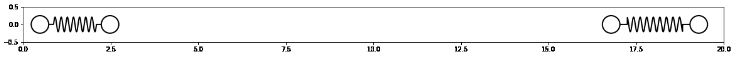
\includegraphics[width=.99\textwidth]{Animation1D.png}
      \caption{Première phase de l'animation. Pour simplifier les choses, le dispositif visqueux comme en \cref{fig:dep1d} n'est pas représenté ici. }
      \label{fig:anim1}
    \end{figure}
    \item \textbf{Après le contact}: la semaine dernière, nous avons calculé les "vitesses initiales" pour cette phase. On se retrouve donc avec un système illustré à \cref{fig:dep1d}. Malheureusement, ce système ne converge que lorsque $v_0 = v'_0$; sinon, les déplacements $x_1$ et $x_2$ explosent vers des valeurs aberrantes (voir notebook "Deplacement1D.ipynb"). Cela pose naturellement problème pour l'animation de la deuxième phase de la percussion. Je suis donc en pleine investigation de cette question.
\end{enumerate}


%----------------------------------------------------------------------------------------
%	ASSIGNMENT CONTENT - SECTION 2
%----------------------------------------------------------------------------------------

\section*{Difficultés rencontrées}

\textit{Le rapport de stage et un notebook Python sont rattachés à ce rapport.}

\begin{enumerate}
  \item La première difficultés était de définir comment animer le modèle et avoir une vue au moins du comportement en 1D (en Python);
  \item La deuxième est que le modèle de déplacements 1D ne converge pas lorsque les deux vitesses de ses extrémités sont d'amplitudes différentes. Analytiquement, j'ai pu calculer la solution lorsque la matrice $E$ (voir rapport de stage, section "1.2.2.1 Modélisation du déplacement d’un floe isolé") est trigonalisable; la solution devrait converger !
\end{enumerate}


%----------------------------------------------------------------------------------------
%	ASSIGNMENT CONTENT - SECTION 3
% ----------------------------------------------------------------------------------------

\section*{Travail à venir}

\begin{enumerate}
  \item Calcul de la solution de modèle de déplacement 1D lorsque la matrice $E$ n'est pas trigonalisable; il faudra intégrer les nombres complexes dans notre étude, et j'essaie en ce moment de trouver comment le faire de la meilleure des manière.
  \item Animation de la deuxième phase de la percussion (après contact).
\end{enumerate}



% %-------------------------------------------------------------------------------
% %							THE BIBLIOGRAPHY
% %-------------------------------------------------------------------------------
\clearpage   % Pour retirer les references de la bare de navigation
\printbibliography


\end{document}
